\chapter{Recommender System}
Recommender system is and remains a hot topic within computer science in 2015. Huge conferences are hosted in different parts of the world annually, featuring many big companies. The RecSys conference [33] is a good example
of this. Recommender Systems has a wide use-area within all kinds of advertisement on the web when specifically targeted ads are needed. These ads can be seen everywhere from websites and apps to emails, text-messages etc. In the list of big actors on the stage of recommender systems, hardly surprisingly, one find companies such as Facebook, Google etc. But Recommender Systems are also used for recommending music in for instance Spotify and movies/TV-shows in Netflix. There are a variety of different algorithms for each use-area. The setting of which this thesis will focus consists in algorithms for recommender systems within garment-based e-commerce. Here follows some of the more common general techniques used in recommender systems.

\cite{Adomavicius2005}
\nocite{Adomavicius2015}
\nocite{Aggarwal2013}
\nocite{Aggarwal2015}
\nocite{Ansari2000}
\nocite{Bobadilla}
\nocite{Bobadilla2013}

\section{Collaborative Filtering}
The basic idea of collaborative filtering is to find information or patterns using collaborative techniques among multiple data sources. Data sources typically consist of users and items such as movies, songs etc. Within e-commerce, and this project specifically, those data sources mainly consist of users, and products that can be bought by these users. Finding these patterns is accomplished through collecting and analysing huge amounts of data on users’ behaviours and activities as well as items. Within e-commerce those activities and behaviours include but are not limited to purchases and click-able ad- vertisements. Collaborative filtering[18] is one of the most common general methods for recommender systems being applicable within several big use-areas. Collaborative Filtering is frequently used in social networks such as Facebook, LinkedIn, mySpace, Twitter etc to effectively recommend new friends, pages, groups as well as who to follow or what to like. But also applications such as Youtube, Reddit, Netflix etc make use of collaborative filtering. Collaborative filtering is viable in all applications where one can observe connections between a user and their registered friends or followers. But it is also widely used within e-commerce, where Amazon is a good example who popularised algorithms for item-to-item based collaborative filtering [21].


The paper discusses the state-of-the-art recommender systems for the current generation. Industry and academia has shown great interest in the field of recommendation systems (RS). Abundant approaches the RS which can be further improved to enhance the capabilities and functionality. Major application in industry has given research a boost and many companies/vendors have incorporated RS in to their commercial servers. Recommender systems have been the major milestones in the application of Computer Science to other areas. This can be categorized into collaborative-filtering, content based RS and some Hybrid Approaches. Content-based RS focuses on building user profile of a single user for recommendations while collaborative-filtering(CF) RS uses data from fellow users/peers to recommend a particular user. Content-based RS has its roots in Information Retrieval, utility function is defined for each item for a user based on the history of the user purchases, searches, etc. Usually, higher the utility function value, higher is the preference for recommendation. Limited feature Extraction leads to limited possible recommendations. Also, only domain specific recommendations can be inferred. New user problem exists for the both kind of the RS systems. Almost no information is present about the new users into the application environment. Collaborative-filtering techniques create user groups/clusters based on similar tastes/browsing habits, and few techniques consider stereotypes for peer groups. And collaborative-filtering is of two types based on the data mining techniques; heuristics (memory) based, model-based CF. Both techniques have decent application in the industry for real world problem solving. Improvements have been shown in the combined use of these data mining techniques.

\begin{figure}[H]
    {\centering {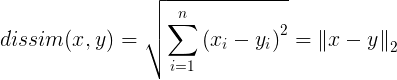
\includegraphics[width = 0.7 \textwidth]{img/DissimEqn.png}}\par}
    \caption{Dissimilarity}
\end{figure}

In memory-based CF, similarity among users is calculated using cosines of the user matrices. Correlation and similarity are calculated by heuristic techniques.Heuristics basically work by aggregation or summation(∑) of the past activities of the users who are similar to a user for whom recommendations are required. Another is Model-based CF, models are prepared based on ANN, K-means clustering, Gibbs sampling, Probabilistic latent semantic analysis, generative semantics of latent Dirichlet Allocation. CF recommendation systems also faces few issues; new item problem, in which recommendations of this new item are not made to any use because of the shortage of the data; Sparsity, this issue arises for a user whose tastes are fairly diverse from the other users which increases hardness of the recommendations. Demographic-based filtering and preference-based filtering could be helpful with these kind of limitations. Preference-based filtering is currently high on research and industry use. Improvements over the limitations of the above RS have been implemented using hybrid RS and many extensions of current RS. Current state of the recommender systems can be enhanced by extending the capabilities of RS. One approach highlighted is use of advanced profiling of items and users. Another by the use of Mathematical Approximation Theory and some RBF. Multidimensionality Reduction based on contextual approaches on recommender systems. Multiple rating criterias which help user to rate an item from various perspectives not just one. Making RS less intrusive to a user of the application system, providing some control to the user for change in the behavior of RS. Improving flexibility of RS, providing language like RQL for handling operations on RS. Measuring how effective RS has been by calculating the results in various fashions. There are many unexplored characteristics of RS which may even lead to other fields of study.

Most Collaborative Filtering techniques can be expressed by the two general steps, Similarity Computation and Prediction Generation, described under 2.2

\subsection{User based collaborative filtering}
The main idea of recommender systems built on user-based collaborative filtering consists in computing the similarity between users’ {u,j} profiles, s u\textsubscript{j} . That is, computing a prediction for the probability of the user u liking a specific item i, consists in computing a rating based on all ratings made by users with similar profiles. All similar profiles contribute to this prediction depending on the similarity factor, s uj [34, 35, 36]. 

\begin{figure}[H]
    {\centering {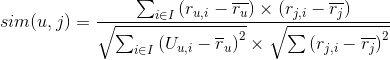
\includegraphics[width = 0.7 \textwidth]{img/PearsonEqn.png}}\par}
    \caption{}
\end{figure}


\begin{figure}[H]
    {\centering {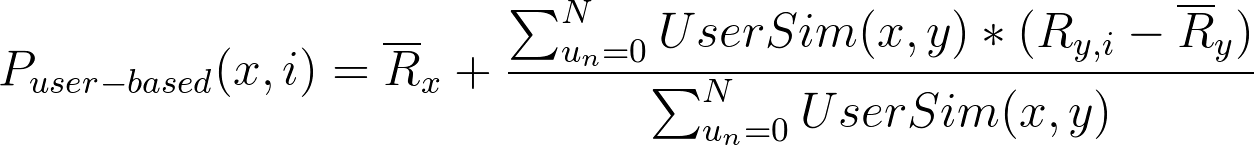
\includegraphics[width = 0.7 \textwidth]{img/PredUserEqn.png}}\par}
    \caption{}
\end{figure}

Typically this can be reduced to the two general steps. 
1. While observing a user’s actions in a system, look for similar users with equal behaviour- and activity-patterns. 
2. Use the observations from step 1 to compute a prediction for the specified user. 

See 2.2 for more information regarding Similarity Computation and Prediction Genera- tion techniques.

\subsection{Item based collaborative filtering}
The concept of item-based collaborative filtering applies the same idea as its User-based counterpart, but the similarity is computed between items instead of users, and is usually described as "Users who bought this also bought that". 

\begin{figure}[H]
    {\centering {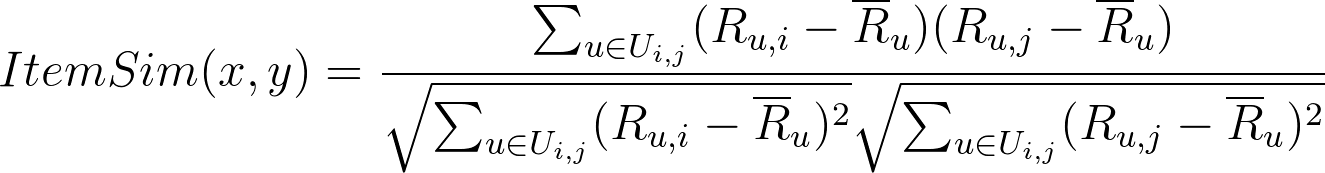
\includegraphics[width = 0.7 \textwidth]{img/ItemSimEqn.png}}\par}
    \caption{}
\end{figure}


\begin{figure}[H]
    {\centering {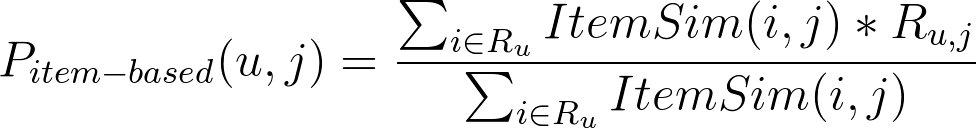
\includegraphics[width = 0.7 \textwidth]{img/PredItemEqn.png}}\par}
    \caption{}
\end{figure}

More generally, taking an item-based approach means looking into the set, I, of items a specific user, u, has rated, using their context to compute the similarity of other items, \{i\textsubscript{0} ,i\textsubscript{1} ,...,i\textsubscript{n} \}, not in I. Their corresponding similarities are computed at the same time as {s i0 ,s i1 ,...,s in }. When these similarities and their corresponding items have been found, a prediction can be computed. [36, 37, 38]. 
This can typically be split into three steps: 
1. Construct a User-Item matrix, M[u][i], giving each index of the matrix a rating, r ui , on an item i performed by a user u. 
2. Compute the similarity, s i\textsubscript{1}, i\textsubscript{2}, of two items i 1 and i 2 by looking at co-rated pairs from different users.
3. Generate predictions based on some prediction method, described under 2.2. Item-based collaborative filtering is a very common approach, often used together with algorithms for matrix factorization.

\subsection{Matrix Factorization}
Matrix factorization is an algebraic operation consisting in factorising a matrix M, meaning finding the matrices M 1 ,M 2 ,...,M 3 such that when they are multiplied, the resulting matrix is M. In collaborative filtering based recommender systems this can be used as a rather simple and very intuitive algorithm for discovering latent features. By constructing a User-Item matrix M, where each index contains a rating r on an item i performed by a user u:

\[  
\label{eq:ratingmatrix} \tag{1}
\textbf{M\textsubscript{u,i}} = \left(
\begin{array}{cccc}
r_{{u_1}{i_1}}&r_{{u_1}{i_2}}& \ldots&r_{{u_1}{i_n}} \\
r_{u_2}{i_1}&r_{{u_2}{i_2}}& \ldots&r_{{u_2}{i_n}} \\
\vdots & \vdots & \ddots & \vdots \\
r_{{u_m}{i_1}}&r_{{u_m}{i_2}}& \ldots&r_{{u_m}{i_n}}
\end{array}
\right)
\]

For example, by limiting the matrix to 4×4 and adding some fictitious values for ratings
where - symbolises yet unrated items, a matrix to be factorised might look something
like \eqref{eq:ratingmatrix}


\[  
\label{eq:numbermatrix}
\textbf{M\textsubscript{u,i}} = \left(
\begin{array}{cccc}
5&1& - &4 \\
3&-&\ldots&3 \\
\vdots & \vdots & \ddots & \vdots \\
2&-& \ldots&4
\end{array}
\right)
\]

Matrix factorisation can be seen as the task of predicting the missing ratings meaning filling in the blanks (-) in matrix \eqref{eq:numbermatrix}. Latent features of items liked by different users might be different types of cloths or accessories which might be a shared interest between some users. So for the matrix, 2.2 above, an assumption regarding how many latent features one wishes to find must be made. Let us assume we want to find k latent features and we have the sets U and I containing all users and all items respectively.

This means finding two matrices, N(\textit{a  |U| × k matrix }) and O(\textit{an  |I| × k  matrix}) which when multiplied approximating M:

\[ M \approx N \times O = \hat{M} \]

Further, using similarity and prediction computing techniques as described under 2.2, the gaps can be filled in and thereby resulting in really good recommendations.

\section{Similarity Calculation and Prediction Generation}
Similarity and prediction computations compose vital parts of collaborative filtering based recommender systems. Something that can be seen in 2.1.1, 2.1.2 and 2.1.3. The similarity computation is performed before the prediction generation and the basic idea is to first isolate users who have rated two different items, and secondly to apply some similarity computation technique between these two items to determine their similarity. There are several ways of computing the similarity but some common methods are Cosine-based Similarity, Correlation-based Similarity and Adjusted Cosine-based Similarity, Jaccard Similarity, Jaro-Winkler Similarity, Sörensen Similarity.
When the similarity computation is completed, it is time for the most important part in a collaborative filtering based recommender system; generating the output in terms of prediction. As for computing the similarity there are a number of techniques to choose from when generating predictions. Some of the more common methods are using regression or the weighted average/weighted sum.

\section{Content Based Filtering}\label{contentfiltering}
Another well known method when implementing recommender systems is content-based filtering[16, 17]. Content-based filtering is commonly used for movie recommendations or within other environments where for instance keywords are used to describe the items of the system. Among the actors of recommendation systems using content-based filtering one can find The Internet Movie Database and other popular websites for movies. The methods of Content-based filtering commonly make use of the correlation between item features and preferences from a user’s profile, as opposed to the collaborative filtering approach that selects items based on the correlation between users with similar profiles. 

For the above to work, the system needs to deploy some learning technique [16, 17] such as Bayesian networks, clustering, decision trees, neural networks, reinforcement learning, Nearest Neighbour etc. The system uses these techniques when observing historical data of users to learn their preferences. The intention is that, after sufficient amounts of data have been observed, the system should be able to predict future behaviour of a specific user.


\subsection{Selecting a (Learning) Model}\label{trainingmodel}
A key component when implementing a recommender system using content-based filtering is choosing a method for how the algorithm should be trained [16, 17], using available data from the system. Using this data to create a model of a user’s preferences and history in the system can be seen as a kind of classification problem. There are several significantly different methods suitable for solving this, some of which are mentioned in \autoref{contentfiltering}.

Which one to choose depend on the setting for which it is going to be used. For instance, Bayesian networks are commonly practical in a setting where knowledge about users change slowly, relative to time needed to construct the model. Clustering techniques on the other hand has a tendency to generate less-personal predictions than other methods[40]. Although, due to the nature of clustering, once the clustering process is complete, the new groups of data to be analyzed are significantly smaller than before and performance, in terms of computation time, are thereby likely to be good. Decision trees have shown a tendency of basing classifications on as few instances as possible. Something that has lead to worse performance in the sense of accuracy[41]. Although with a smaller number of structured attributes, the performance and simplicity of decision trees are all advantages when applied in content-based recommender systems. Nearest Neighbour methods are commonly known as old and reliable go-to methods when nothing else works. It has the worst performance in most cases, but are most likely to succeed[17].

\section{Demographic Filtering}
Recommender systems built around the concept of demographic filtering work very much like their content-based counterpart, although only making use of personal data provided by the users themselves through a registering process, survey response, purchase history etc. This rather than observing and learning user behaviour to classify the users depending their purchase history, ratings etc[20, 42]. A Demographic filtering approach does not, in contrary to content-based filtering, apply a user preference model. It does however apply an item preference model for the items of a system. This basically means that a demographic approach is more privacy-preserving than a content-based filtering one[19].

\section{Other recommendations techniques}
The techniques described under 2.1, 2.3 and 2.4 are the most common when implementing recommender systems [20, 43]. More approaches have been studied and considered, but none that are to be considered more common than the ones described in 2.1, 2.3 and 2.4. One example is using techniques of knowledge-based filtering described in[44].

\section{Hybrid Recommender Systems}
A hybrid approach to implementing recommender system means designing the system so as to making use of several recommendation techniques such as for instance collaborative filtering techniques and content based filtering, making predictions from the combined conclusions of the two. This can be done by unifying the two techniques, by adding features from one into the other or simply by running algorithms for both techniques separately and then combine the results in some way. The most common example of a hybrid based recommender system is the one used by Netflix. While an environment like Netflix is well suited for a hybrid recommender system, it does not fit everywhere.

Why Netflix is considered a hybrid system:

\begin{itemize}
	\item {\textit{Collaborative Filtering}: Observing the watching and browsing habits of similar users.}
	\item {\textit{Content-Based Filtering}: Observing users with equal preferences and how they rated certain movies.}

\end{itemize}

\section{Implementation Challenges in Recommender Systems}

\subsection{Grey/Black Sheep}
These terms ”grey sheeps”, ”black sheeps” are used to refer to the users in the recommender systems. Grey sheep refer to user whose characteristics do not overlap with any other user or group of users, that is not consistently agreeing or disagreeing with any other group of users. Black sheep on the other hand refer to users with extremely varying taste patterns. Something that make predictions nearly impossible.

\subsection{Sparsity and Subjective Problems}
The sparsity problem applies in collaborative filtering based system when it is hard to find items rated by enough people to be feasible to consider (The item-user Matrix is very large and sparse). This is common as the amount of items in most recommender environments exceeds the amount a user is able to explore by far. However sparsity problems in different forms might also be encountered in systems based on content-based filtering. Algorithms for that technique cannot see information as objective or subjective, meaning it cannot distinguish between for instance irony and actual opinions. Which in turn means that a learning algorithm might draw faulty conclusions.


\subsection{Shilling attacks}
In recommender systems where actual ratings constitutes the core of predictions, it is often necessary to introduce precautions to discourage manipulation attempts. These kinds of manipulations might occur in systems where everyone can make ratings, whereas biased users might give lots of positive feedback for products related to themselves and unjustified negative feedback for their competitors.

\subsection{Cold Start}
In a system based on collaborative filtering, new items with no ratings will most likely not be predicted for anyone until it has been rated by several users. The same applies to new users of a specific system. If users do not have any recorded activities on which to base predictions, most recommendations will most likely be inaccurate. Likewise a content-based filtering system will have issues suggesting accurate recommendations of items that the behaviour of a user do not provide evidence for. Additional techniques need to be added to give the recommender system capabilities for solving this.

\subsection{Lack of computational power}
A common challenge when implementing algorithms for collaborative filtering-based recommender systems is the lack of computational power on a single machine whereas most will suffer from scalability problems. Something that is easily understood by imagining that there are systems containing millions of items and even more users, meaning that even algorithms with polynomial or even linear time complexity will be slow. For instance in online environments where recommendations need to be done in real time, without any offline computations, and 2-3 seconds are already too slow.

\subsection{Equal items with different names}
In many systems with millions of items it is pretty common that the same or similar items exist several times in the database, but still have different names or even same names but different ids. Unless thought about, this could be a problem in many recommender systems as they would be treated as different items.

\subsection{The Exploration VS Exploitation dilemma}
A returning issue when working with implementing recommender systems is the exploration versus exploitation trade-off which can be seen mostly in machine-learning environments and is something that every developer needs to consider. Exploration is the task of acquiring new knowledge about an environment or setting while exploitation means using existing knowledge to make decisions or predictions. The dilemma consists in balancing these tasks over time i.e. is it worth risking more exploration for a better reward rather than exploiting already sufficient knowledge about the environment and thereby already getting a good reward with some probability.

And what does this mean when implementing recommender systems for use within ecommerce? An example would be if, let us for simplicity, say that an algorithm used by a recommender system has found one or perhaps a few products that get sold with a high probability every time they are recommended to some type of users. This probability is likely to decrease over time, but how does the algorithm know when to stop recommending the products with known decent profit in favour of exploring new products?

